\documentclass[10pt]{beamer}

%%%
% PREAMBLE FOR THIS DOC 
%%%
%https://tex.stackexchange.com/questions/68821/is-it-possible-to-create-a-latex-preamble-header
\usepackage{/Users/miw267/Repos/latex_preamble/beamer_preamble}



%%% TRY TO RESHOW TOC AT EACH SECTION START (with current section highlighted)
% Reference: https://tex.stackexchange.com/questions/280436/how-to-highlight-a-specific-section-in-beamer-toc
\newcommand\tocforsect[2]{%
  \begingroup
  \edef\safesection{\thesection}
  \setcounter{section}{#1}
  \tableofcontents[#2,currentsection]
  \setcounter{section}{\safesection}
  \endgroup
}


%%%% HERES HOW TO DO IT CORRECTLY
% FIRST IN .STY FILE, DO
%\usetheme[sectionpage=none]{metropolis}
% THEN AT EACH SECTION DO
%\begin{frame}{Outline}
%  \tableofcontents[currentsection]	
%\end{frame}



%\setbeamertemplate{navigation symbols}{}
%\setbeamertemplate{footline}[frame number]{}


%%%
% DOCUMENT
%%%

\begin{document}

%\maketitle

%% Title page frame
%\begin{frame}
%    \titlepage 
%\end{frame}





\title{10/23/2026: Real-valued functions of real variables}
\author{CSCI 246: Discrete Structures}
\date{Textbook reference: Chap 11.1, Epp}

\begin{frame}
    \titlepage 
\end{frame}


\begin{frame}
%\footnotesize 
%\begin{mygreenbox}[title=Graded Quiz Pickup]
%Quizzes are in the front of the room, grouped into four bins (A-G, H-L, M-R, S-Z) by last name. The quizzes are upside down with your last name on the back. Come find yours before, during, or after class.  Only turn the quiz over if it's yours.
%\end{mygreenbox} 
%\vfill 

%\begin{myredbox}[title=Announcements]
%\begin{itemize}
%	\item Please sign the sign-in sheet.
%	%\item \red{TODO: Update}
%\end{itemize}

%\end{myredbox}

\vfill 


\begin{myyellowbox}[title=Today's Agenda]
\begin{itemize}
	\item Quiz ($\approx$ 30 mins)
	\item Group exercises ($\approx$ 20 mins)
\end{itemize}

%	
\end{myyellowbox}
\vfill 

\end{frame}


\begin{frame}{Quiz 7}

Answer any two questions below for full credit.  Answer a third question for extra credit.
\begin{enumerate}
\item Prove by smallest counterexample that $n < 2^n$ for all $n \in \mathbb{N}$.	
\item Show by induction that $f_0 + \cdots + f_n = f_{n+2} -1$ in the Fibonacci sequence.	
\item Let $a$ be the sequence $0,2,7,15,26,40,57,\hdots$. Write a formula expressing $a_n$ (the $n$-th term in the sequence) as a polynomial function of $n$.
\end{enumerate}


\colorbox{green!30}{\textbf{Definition.}} The \textbf{Fibonacci sequence} is the sequence given by the following recursive rules:
\[f_0 =0, \qquad \quad f_1 =1, \qquad \quad f_{n+2} = f_n + f_{n+1} \]
%The sequence is: $0,1,1,2,3,5,8,13,21,34, \hdots$.

\begin{center}
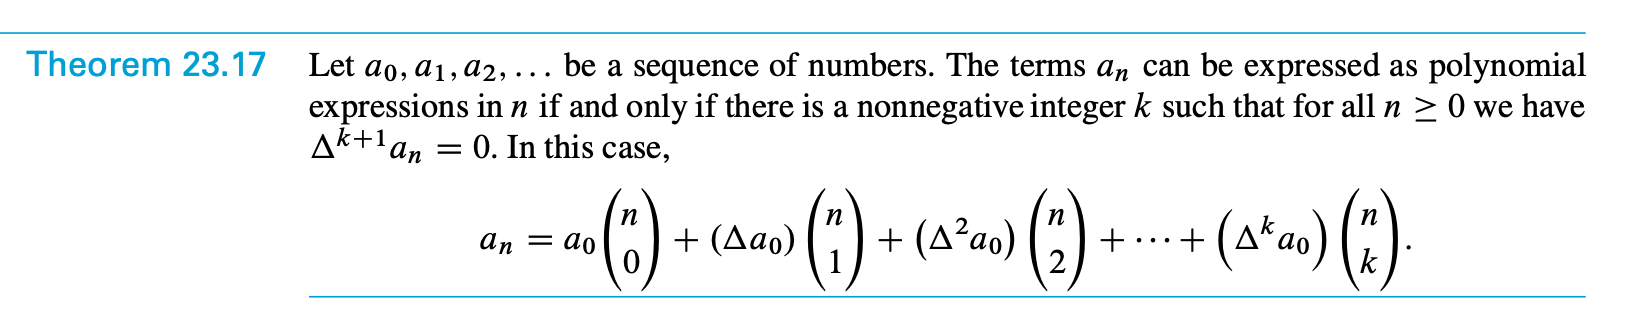
\includegraphics[width=\textwidth]{images/theorem.png}	
\end{center}


\end{frame}


\begin{frame}{Today's goal}

We'll prepare for the section on \alert{computational complexity}, which lets us compare algorithms in terms of how their computational costs grow as a function of input size.  \pause This tells us about \textbf{\texttt{scalability}}.
\vfill 
\pause
The main tool we will use is called Big-O. 
\vfill 
\pause 
Big-O is just careful reasoning about which function is bigger, eventually, up to a constant factor. 
\vfill 
\pause 
Today’s exercises practice each of these pieces: which is bigger (1, 2, 6), eventually (1, 6), and up to a constant (5).
\vfill 
\pause 
\colorbox{blue!30}{\textbf{Remark.}} For this part of the course, we'll temporarily work with real numbers $\mathbb{R}$:
\begin{itemize}
	\item Lets us handle continuous variables (like runtime).  
	\item Big-O notation is typically defined with real numbers so that tools from calculus can be used (like derivatives and limits). \pause However, we won't use calculus tools in this course.
\end{itemize}

\end{frame}


\begin{frame}{Random group assignments}

\begin{columns}
\begin{column}{0.33\textwidth}
Ashley, Isabelle: 4 \\ 
Bailey, Tanna: 6 \\ 
Blaisdell, Olyver: 12 \\ 
Brown, Ashton: 9 \\ 
Cardenas, Dominic: 5 \\ 
Cutler, George: 11 \\ 
Fabik, Roland: 6 \\ 
Fellows, Audrey: 10 \\ 
Fitzgerald, Ryan: 4 \\ 
Fuller, Ryan: 7 \\ 
Griffen, Clara: 9 \\ 
Grutsch, Tanner: 1 \\\end{column}
\begin{column}{0.33\textwidth}
Hager, Nathan: 11 \\ 
Horner, Jayden: 12 \\ 
Johnson, Jaret: 6 \\ 
Kintzel, Samantha: 7 \\ 
Lameres, Alexis: 1 \\ 
Lee, Holden: 4 \\ 
Mayala, Reece: 3 \\ 
McLean, Connor: 8 \\ 
Mcbride, Daniel: 8 \\ 
Miller, Maverick: 10 \\ 
Moss, Emily: 2 \\ 
Mousseau, Matthew: 11 \\\end{column}
\begin{column}{0.33\textwidth}
Neuman, Evan: 12 \\ 
Putnam, John: 2 \\ 
Ramos, Vydel: 3 \\ 
Rathbun, Jedidiah: 2 \\ 
Roberts, Matthew: 10 \\ 
Roller, Nathan: 1 \\ 
Ryan, Otis: 9 \\ 
Shevtsov, Timothy: 8 \\ 
Stensland, Emma: 5 \\ 
Thiessen, Logan: 3 \\ 
Thompson, Jaiden: 5 \\ 
Vath, Ethan: 7 \\\end{column}
\end{columns}

	
\end{frame}



\begin{frame}{Group exercises} 
\footnotesize 
\begin{enumerate}	
\item Sketch the graphs of the power functions $p_{2}$ and $p_{3}$ on the same set of axes.
	\begin{enumerate} \footnotesize 
	\item[a.]  When $x>1$, which is greater, $x^{2}$ or  $x^{3}$?
	\item[b.] When $0<x<1$, which is greater, $x^{2}$ or  $x^{3}$?
		\end{enumerate}
\item Repeat the above problem for $p_{1/2}$ and $p_{1/3}$. 
\item The graph of the function $f$ is shown below. Find the intervals on which $f$ is increasing and the intervals on which $f$ is decreasing.
\begin{center}
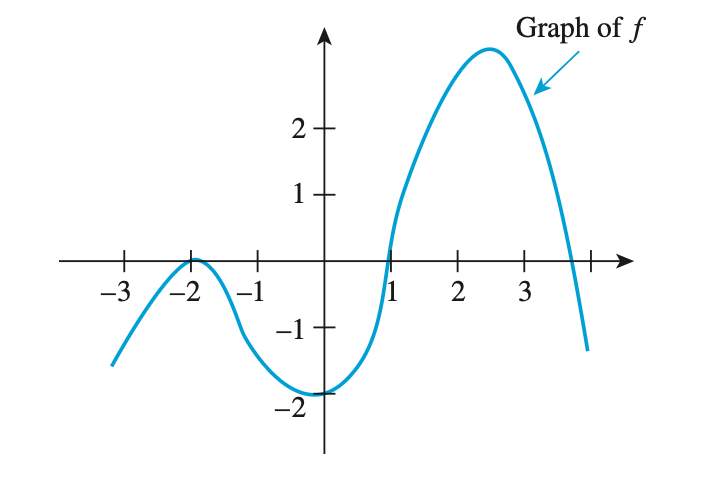
\includegraphics[width=.35\textwidth]{images/group_exercise_plot.png} 
\end{center}
\item Show that if a function $f: \R \to \R$ is increasing, then $f$ is one-to-one.
\item Let $f$ be a real-valued function of a real variable. Show that if $f$ is decreasing on a set $S$ and if $M$ is any positive real number, then $Mf$ is decreasing on $S$.
\item Let $h$ be a function from $\R$ to $\R$ defined by the formula $h(x) =x^2$ for each real number $x$.
	\begin{enumerate} \footnotesize 
	\item[a.] Show that $h$ is decreasing on the set of real numbers less than zero.
	\item[b.]  Show that $h$ is increasing on the set of real numbers greater than zero.
	\end{enumerate}
\end{enumerate}
\end{frame}

\begin{frame}{Solution to group exercise \#1} 
\textbf{Problem.}  Sketch the graphs of the power functions $p_{2}$ and $p_{3}$ on the same set of axes.
	\begin{enumerate} \footnotesize 
	\item[a.]  When $x>1$, which is greater, $x^{2}$ or  $x^{3}$?
	\item[b.] When $0<x<1$, which is greater, $x^{2}$ or  $x^{3}$?
		\end{enumerate}


\vfill 
\textbf{Solution.} 

\begin{center}
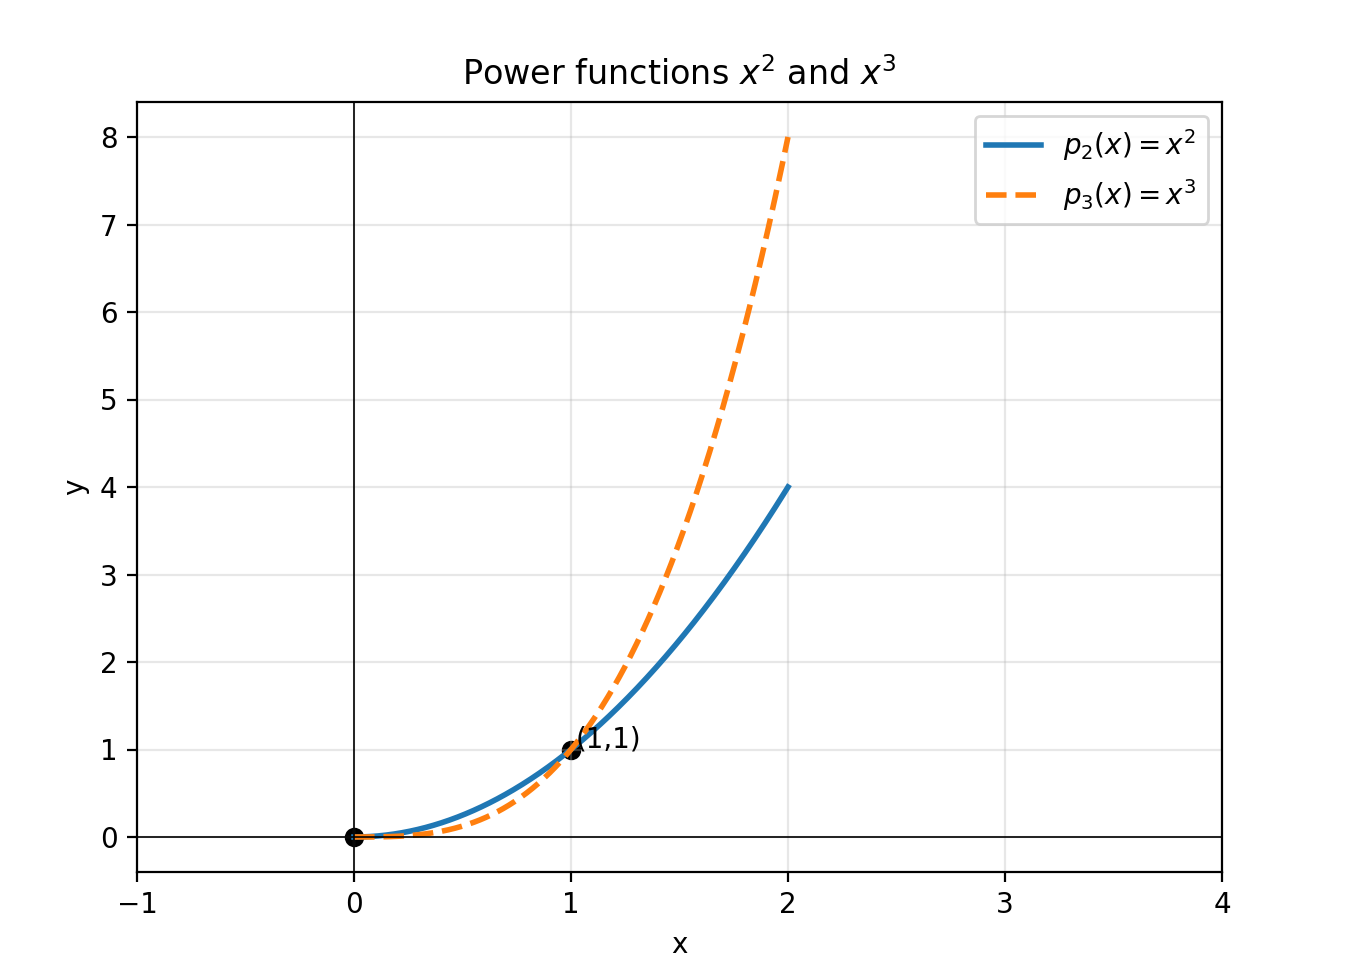
\includegraphics[width=.5\textwidth]{images/solution_to_group_exercise_1.png} 
\end{center}
\footnotesize 
a. $x^{3}$. This happens because multiplying by  x (which is greater than 1) repeatedly makes the result larger each time. b. $x^{2}$. This happens because multiplying by  x (which is less than 1) repeatedly makes the result smaller each time. 

\end{frame}

\begin{frame}{Solution to group exercise \#2} 
\textbf{Problem.}  Sketch the graphs of the power functions $p_{1/2}$ and $p_{1/3}$ on the same set of axes.
	\begin{enumerate} \footnotesize
	\item[a.]  When $x>1$, which is greater, $x^{1/2}$ or  $x^{1/3}$? 
	\item[b.] When $0<x<1$, which is greater, $x^{1/2}$ or  $x^{1/3}$?

	\end{enumerate}


\vfill 
\textbf{Solution.} 

\begin{center}
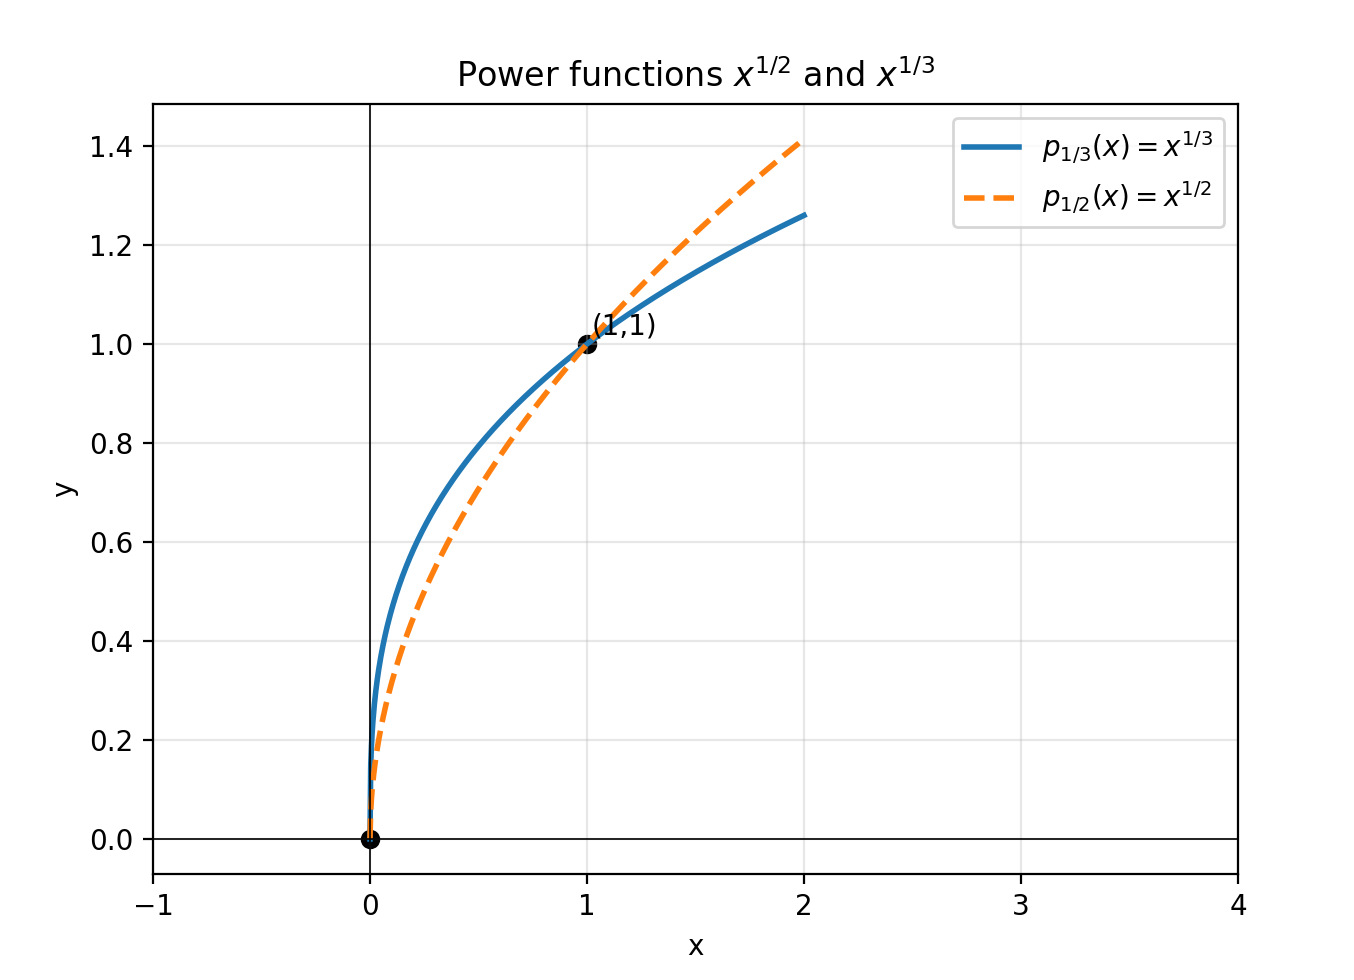
\includegraphics[width=.5\textwidth]{images/solution_to_group_exercise_2.png} 
\end{center}
\footnotesize 
%a. $x^{1/2}$. This happens because multiplying by  x (which is greater than 1) repeatedly makes the result larger each time. b. $x^{1/3}$. This happens because multiplying by  x (which is less than 1) repeatedly makes the result smaller each time. 
a. $x^{1/2}$. \; b. $x^{1/3}$. \; \textit{Why?} Write $x^{1/2} = x^{1/3} \cdot x^{1/6}$. If $x>1$, then $x^{1/6} > 1$, so multiplying by it makes $x^{1/3}$ larger. If $0<x<1$, then $0 < x^{1/6} < 1$, so multiplying by it makes $x^{1/3}$ smaller.
\end{frame}


\begin{frame}{Solution to group exercise \#3} 
\textbf{Problem.} The graph of the function $f$ is shown below. Find the intervals on which $f$ is increasing and the intervals on which $f$ is decreasing.
\begin{center}
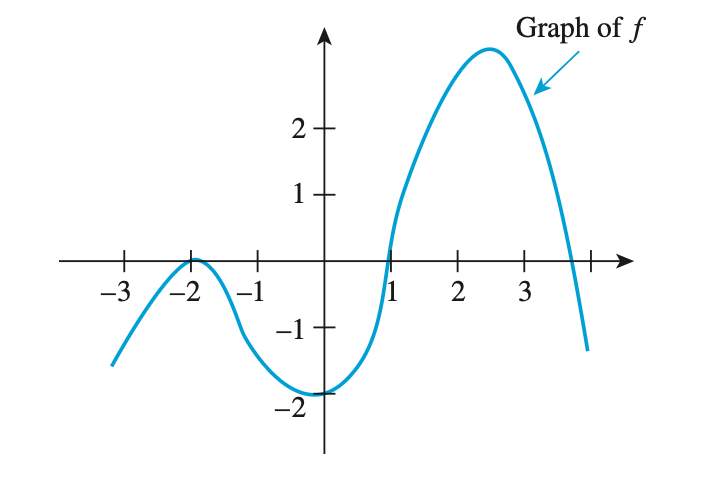
\includegraphics[width=.6\textwidth]{images/group_exercise_plot.png} 
\end{center}

\vfill 
\textbf{Solution.} 
The function $f$ is
\begin{itemize}
	\item increasing on $(-3,-2)$ and $(0,2)$, and
	\item decreasing on $(-2,0)$ and $(2,4)$.
\end{itemize}
\end{frame}


\begin{frame}{Solution to group exercise \#4}
\textbf{Problem.} Show that if a function $f: \R \to \R$ is increasing, then $f$ is one-to-one.
\vfill 
\textbf{Solution.} We want to show that $f$ is one-to-one.   That is, we want to show that that distinct inputs lead to distinct outputs: if $x \neq y$, then $f(x) \neq f(y)$.   Now since $x$ and $y$ are real numbers, if $x \neq y$, then either $x<y$ or $y>x$. So since $f$ is increasing, either $f(x)<f(y)$ or $f(y)>f(x)$. Either way, $f(x) \neq f(y)$.	
\end{frame}


\begin{frame}{Solution to group exercise \#5}
\textbf{Problem.} Let $f$ be a real-valued function of a real variable. Show that if $f$ is decreasing on a set $S$ and if $M$ is any positive real number, then $Mf$ is decreasing on $S$.
\vfill 
\textbf{Solution.} We have that for all $x,y \in S$,
\[ x < y \implies f(x) > f(y) \implies Mf(x) > Mf(y),\]
where the first implication holds since $f$ is decreasing on $S$, and the second implication holds since multiplication by a positive number preserves the direction of an inequality.

Hence, $Mf$ is decreasing.
\end{frame}

\begin{frame}{Solution to group exercise \#6}
\textbf{Problem.} Let $h$ be a function from $\R$ to $\R$ defined by the formula $h(x) =x^2$ for each real number $x$.
	\begin{enumerate} \footnotesize 
	\item[a.] Show that $h$ is decreasing on the set of real numbers less than zero.
	\item[b.]  Show that $h$ is increasing on the set of real numbers greater than zero.
	\end{enumerate}

\vfill 
\textbf{Solution.}	
	\begin{enumerate} \footnotesize 
	\item[a.] Let $x,y <0$ with $x<y$. Multiplying $x<y$ by $x$ and by $y$ (both negative, so each reverses the inequality) gives
\[ x^2 > xy \qquad \text{and} \qquad xy > y^2. \]
Chaining these, $x^2 > xy > y^2$, so $h(x) > h(y)$. Hence $h$ is decreasing on the negative real numbers.
	\item[b.] Let $x,y >0$ with $x<y$. Multiplying $x<y$ by $x$ and by $y$ (both positive, so each preserves the inequality) gives
\[ x^2 < xy \qquad \text{and} \qquad xy < y^2. \]
Chaining these, $x^2 < xy < y^2$, so $h(x) < h(y)$. Hence $h$ is increasing on the positive real numbers.

	\end{enumerate}
\end{frame}


\end{document}
